\section{Dispersal-Extinction-Cladogenesis model}

\subsection{Motivation}

XXX

\subsection{Model and method}

This section contains a brief description of the data, model, parameters, and method used in BayArea.

First, we define the range for taxon $i$ as the bit vector $X_i$, where $X_{i,j} = 1$ if the taxon is present in area $j$ and $X_{i,j} = 0$ if the taxon is absent.
Each taxon range is a bit vector of length $N$ areas.
For example, if taxon $B$ is present only in areas 2 and 3 out of $N=3$ areas, its range is represented as $X_B = (0,1,1)$, which is translated to the bit string $X_B=011$ for short.
If we apply the labels A, B, and C to our three areas, this bit vector can also be represented as a set: $X_B=011$ is the same as $X_B = \{ B, C \}$, or $X_B=BC$ for short.
The data matrix, $\textbf{X}$, is analogous to a multiple sequence alignment where each element in the data matrix reports a discrete value for a homologous character shared by all taxa at column $j$.

\subsection{Modeling anagenic range evolution}

Next, we need a model of anagenic range evolution.
Since we have discrete characters we'll use the continuous-time Markov chain, which allows us to compute transition probability of a character changing from $i$ to $j$ in time $t$ through matrix exponentiation
\[
\mathbf{P}_{i,j}(t) = \left[ \exp \left\lbrace \mathbf{Q}t \right\rbrace \right]_{i,j},
\]
where $\textbf{Q}$ is the instantaneous rate matrix defining the rates of change between all pairs of characters, and $\textbf{P}$ is the transition probability rate matrix.
This technique of matrix exponentiation is powerful because it integrates over all possible scenarios of character transitions that could occur during $t$ so long as the chain begins in state $i$ and ends in state $j$. Remember, $i$ and $j$ represent different ranges, each of which is encoded as a set of occupied areas.

We can then encode range evolution events into the allowed character transitions of $\textbf{Q}$ and parameterize the events so that we may infer their relative importance to generating our observed ranges.
We'll take a simple model of range expansion (e.g. $BC \rightarrow ABC$) and range contraction (e.g. $BC \rightarrow C$).
(Range expansion may also be referred to as dispersal or area gain and range contraction as extirpation or area loss.)
The rates in the transition matrix for three areas might appear as

\[
\textbf{Q} = 
	\begin{array}{c|cccccccc}
		& \emptyset & A & B & C & AB & AC & BC & ABC \\
		\hline
		\emptyset & - & 0 & 0 & 0 & 0 & 0 & 0 & 0 \\
		A & e_A & - & 0 & 0 & d_{AB} & d_{AC} & 0 & 0 \\
		B & e_B & 0 & - & 0 & d_{BA} & 0 & d_{BC} & 0 \\
		C & e_C & 0 & 0 & - & 0 & d_{CA} & d_{CB} & 0 \\
		AB & 0 & e_B & e_A & 0 & - & 0 & 0 & d_{AC} + d_{BC} \\
		AC & 0 & e_C & 0 & e_A & 0 & - & 0 & d_{AB} + d_{CB} \\
		BC & 0 & 0 & e_C & e_B & 0 & 0 & - & d_{BA} + d_{CA} \\
		ABC & 0 & 0 & 0 & 0 & e_C & e_B & e_A & - \\								
	\end{array},
\]
where $e = ( e_A, e_B, e_C )$ are the (local) extinction rates per area, and $d = ( d_{AB}, d_{AC}, d_{BC}, d_{CB}, d_{CA}, d_{BA})$ are the dispersal rates between areas.

{\bf Q: For the three-area DEC rate matrix above, what is the rate of leaving state 101? That is, what is the absolute value of the diagonal term in the rate matrix for $Q_{AB,AB}$? }

Note the rate of more than one event occurring simultaneously is zero, so a range must expand twice by one area in order to expand by two areas.

{\bf Q: What events might explain a transition from range $ABC$ to range $A$? From range $AB$ to range $C$?}

Of course, this model can be specified for more than three areas.

{ \bf Q: Imagine a DEC rate matrix with four areas, $ABCD$. What would be the dispersal rate for $Q_{BC,BCD}$? How many states does a DEC rate matrix with four areas have? What is the relationship between the number of areas and the number of states under the DEC model? }

Let's consider what happens to the size of \textbf{Q} when the number of areas, $N$, becomes large.
For three areas, \textbf{Q} is size $8 \times 8$.
For ten areas, \textbf{Q} is size $2^{10} \times 2^{10} = 1024 \times 1024$, which approaches the largest size matrices that can be exponentiated in a practical amount of time.
For biogeographic inference under large numbers of areas, see the Tutorial XXX \citep{landis13}.


\subsection{Modeling cladogenic range evolution}

In addition to dispersal and extinction, the DEC models cladogenic range evolution events.
For each internal node in the reconstructed tree, one of two cladogenic events can occur: sympatry or allopatry.
Say the range of a species approaching an internal node, i.e. that is about to speciate, is $A$.
Since the species range is size one, this always results in sympatry, where both daughter lineages inherit the ancestral species range, so both lineages begin in state $A$.
The notation $A \rightarrow A \mid A$ describes this event: the state is $A$ before cladogenesis, the left daughter inherits range $A$ after cladogenesis, as does the right daughter.

Now suppose the ancestral range is $ABC$.
Under sympatric cladogenesis, one lineage identically inherits the ancestral species range, $ABC$, while the other lineage inherits only a single area, i.e. only $A$ or $B$ or $C$.

Under allopatric cladogenesis, the ancestral range is split evenly among daughter lineages, e.g. one lineage may inherit $AB$ and the other inherits $C$.
Both daughter lineages inherit the entire ancestral species range following widespread sympatric cladogenic events.
For a general description of state transitions for cladogenic events, see \citet{matzke13}.

{\bf Q: What are the 6 possible states in the daughter lineages after cladogenesis given the state is $AB$ before cladogenesis?}

The probabilities of anagenic change along lineages must account for all combinations of starting states and ending states.
For 3 areas, there are 8 states, and thus $8 \times 8 = 64$ probability terms for pairs of states.
For cladogenic change, we need transition probabilities for all combinations of states before cladogenesis, after cladogenesis for the left lineage, and after cladogenesis for the right lineage.
Like above, for three areas, there are 8 states, and $8 \times 8 \times 8 = 512$ cladogenic probability terms.

{\bf Q: For three areas, there are 3 + 12 + 6 = 21 possible sympatry events and 6 + 6 = 12 possible allopatry events. How many terms in the cladogenesis matrix are zero?}

The DEC model ignores speciation events hidden by extinction or incomplete taxon sampling.
The probability of cladogenesis and local extinction events would ideally be linked to a birth-death process, as it is in the GeoSSE model \citep{goldberg11}.
Unfortunately, since this sort of model scales poorly, and DEC models remain the only option when the geography has more than two or three areas.


\begin{figure}[H]
\centering
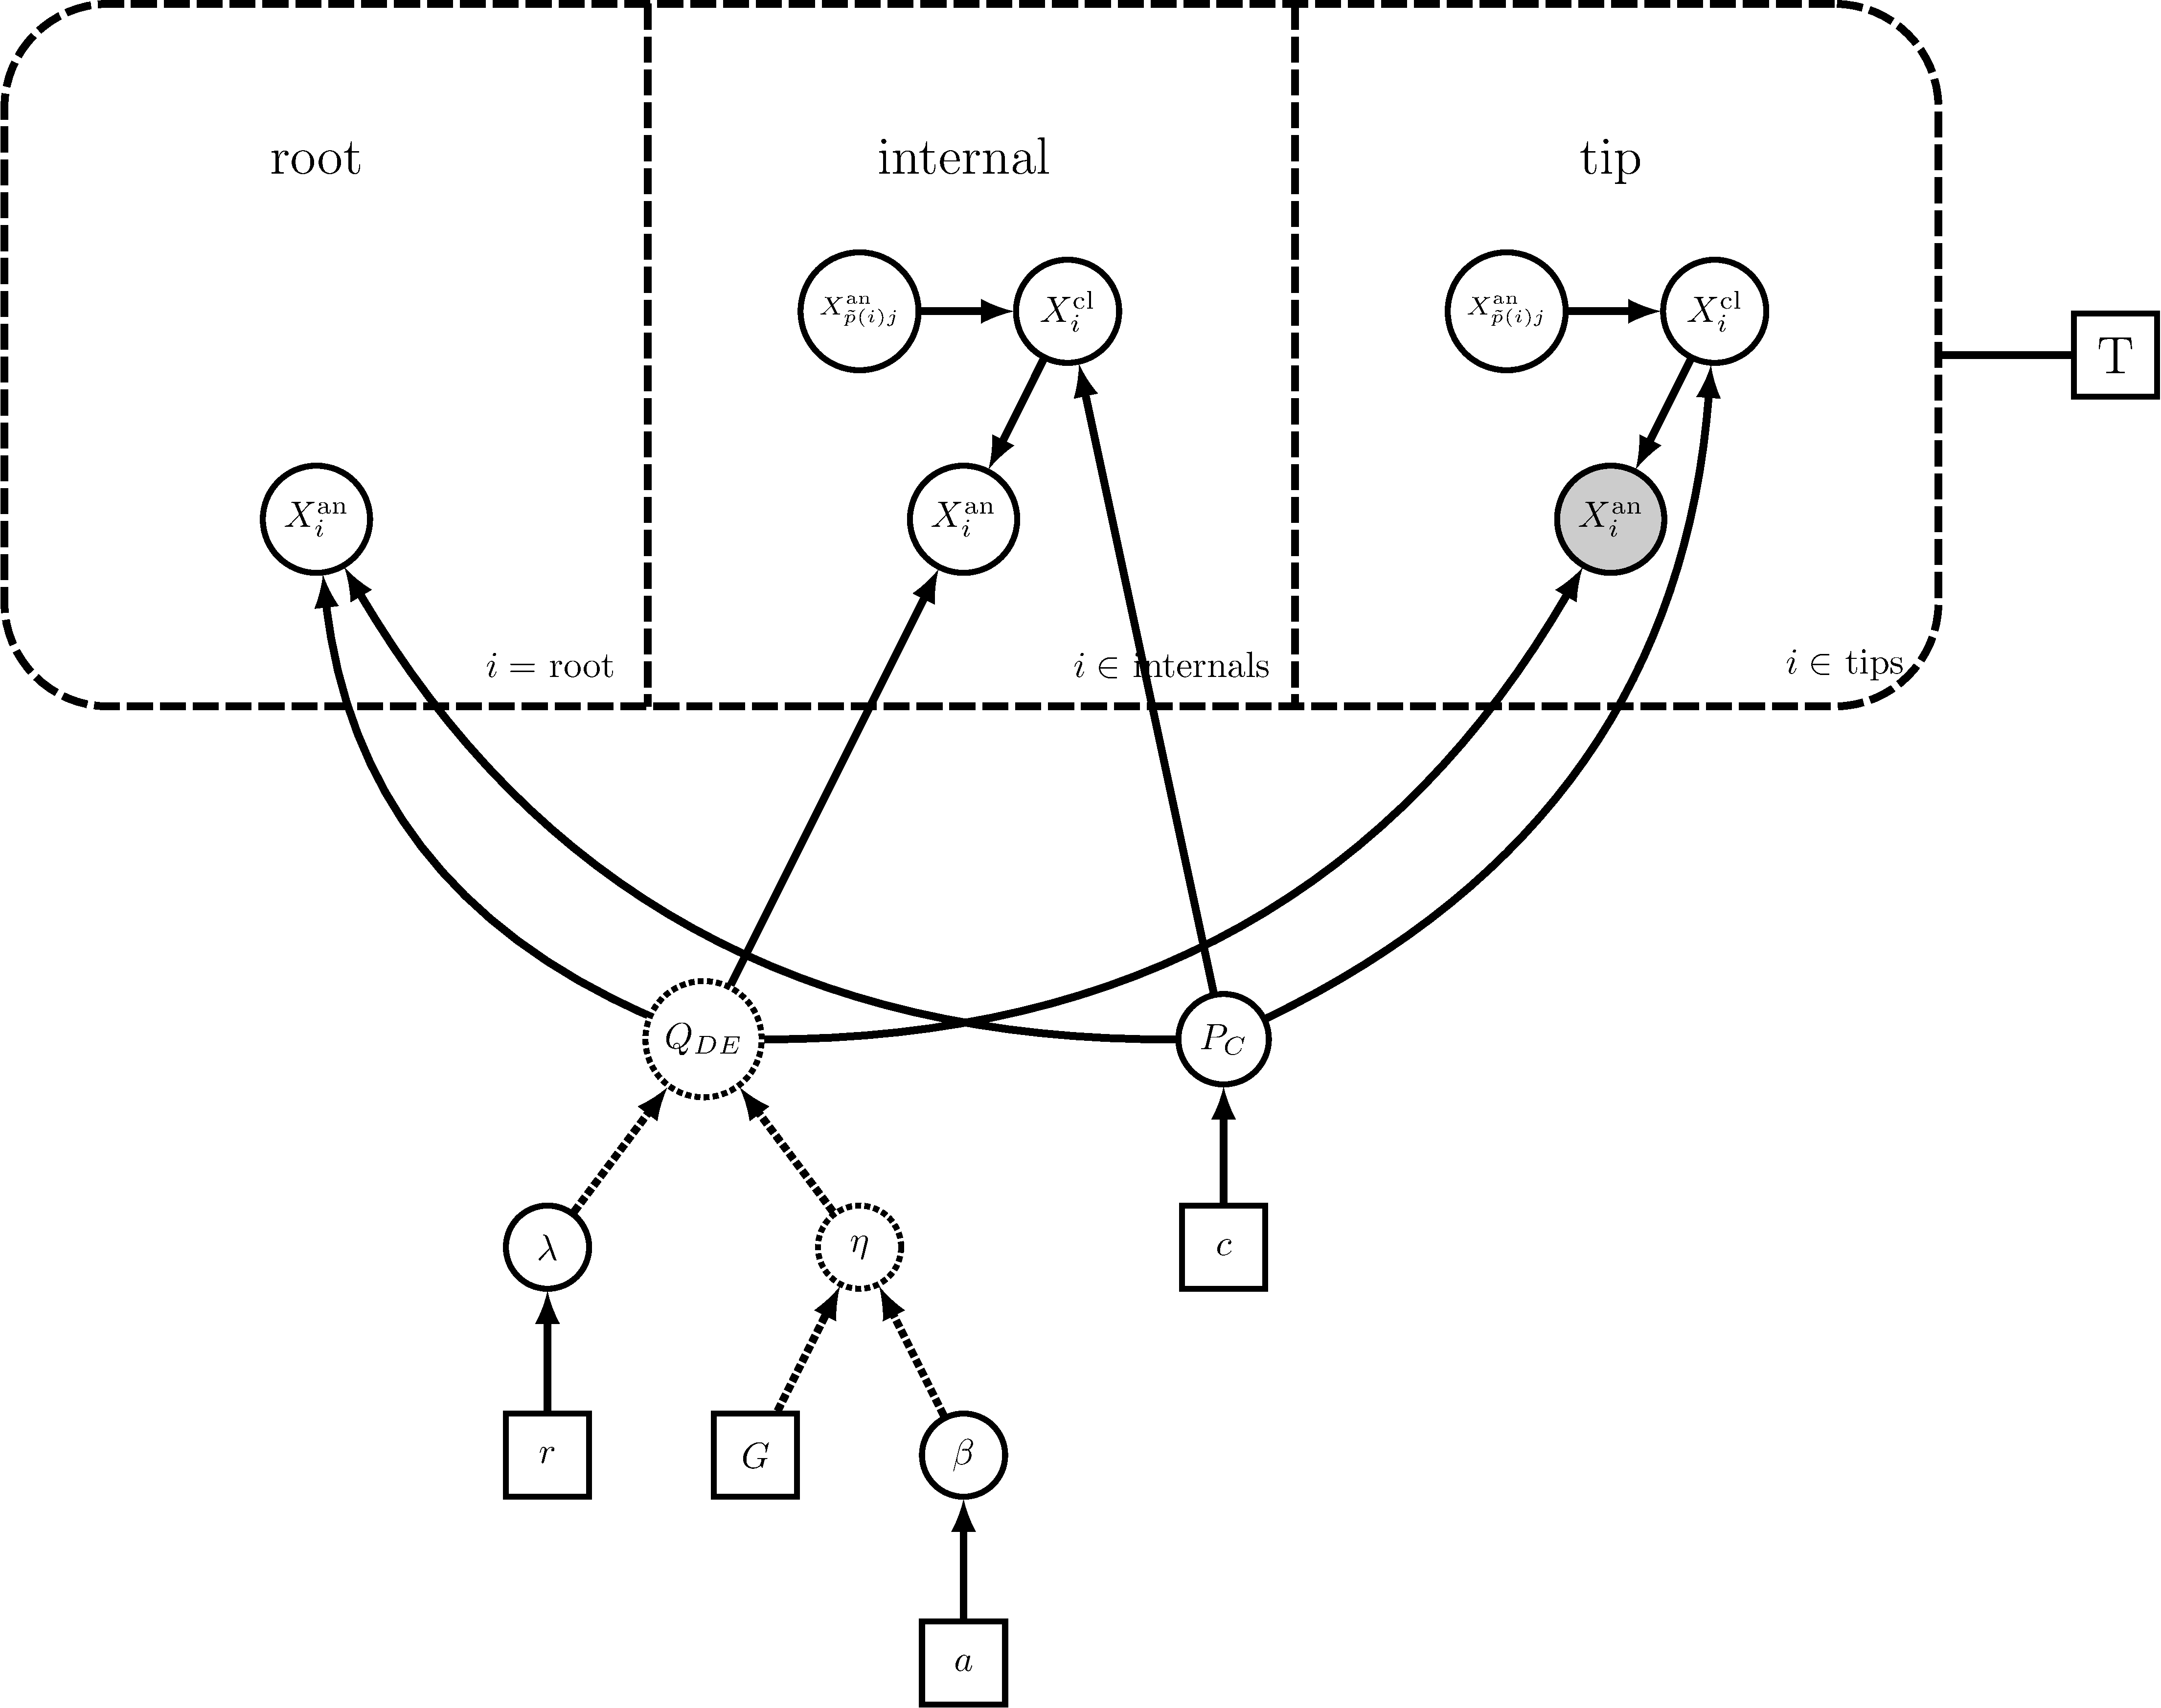
\includegraphics[width=5in]{figures/bg_dec_dag}
\caption{Graphical model of DEC. The tree plate's topology is fixed by $T$, where each internal node has both an anagenic and cladogenic random variable ($X_i^{\text{an}}$ and $X_i^{\text{cl}}$, resp.) that represents an ancestral species before and after it speciated. Anagenic change is modeled by a continuous time Markov process, where $Q_{DE}$ is the instantaneous rate matrix of area gain and loss, as parameterized by $\lambda$. The geographic distance rate modifier function, $\eta$, takes in the geographical distances and strata as $G$, and the distance power parameter, $\beta$. Cladogenic change is modeled by $P_C$, a Dirichlet-distributed simplex with a flat prior.}
\end{figure}

The rest of this tutorial will describe how to run a simple DEC analysis using RevBayes.

\newpage

%%%%%%%%%%%%%%%%
%%%%%%%%%%%%%%%%

\subsubsection{Specifying a simple DEC model}

We'll use a dataset for XXX primates whose ranges are over three areas: Africa, Eurasia, and the New World.
Read in the dataset



\begin{snugshade}
\begin{lstlisting}

\end{lstlisting}
\end{snugshade}


For simplicity, we'll assume

First we'll create some {\tt String} variables for file handling

\begin{snugshade}
\begin{lstlisting}
fp = "/Users/mlandis/projects/revbayes_tutorial/RB_Biogeography_DEC_tutorial/"
data_fn = fp + "data/primates_bg_n3.tsv"
tree_fn = fp + "data/primates_tree.tre"
\end{lstlisting}
\end{snugshade}

then read in our character data

\begin{snugshade}
\begin{lstlisting}
d = readTSVCharacterData(data_fn, type="NaturalNumbers")
\end{lstlisting}
\end{snugshade}

Next, compute the number of states from the number of areas

\begin{snugshade}
\begin{lstlisting}
n_areas = d.nchar()
n_states = 2^d.nchar()
\end{lstlisting}
\end{snugshade}

We assume the tree is known from an independent time calibration analysis

\begin{snugshade}
\begin{lstlisting}
t <- readTrees(tree_fn)[1]
\end{lstlisting}
\end{snugshade}


Declare index variables for our move and monitor vectors for future use

\begin{snugshade}
\begin{lstlisting}
mvi = 1
mni = 1
\end{lstlisting}
\end{snugshade}


Next, we'll begin to construct the rate matrix for anagenic events.

First create a matrix, 8-by-8 in size, initialized with all zeroes

\begin{snugshade}
\begin{lstlisting}
for (i in 1:8) {
    for (j in 1:8) {
        r[i][j] <- 0.
    }
}
\end{lstlisting}
\end{snugshade}

Now we need to populate the non-zero rate matrix elements, which are in terms of dispersal and extinction rates.

For this exercise, we'll use one dispersal rate and one extinction rate, and wait until later to relax this assumption.

First, create a extinction rate parameter and assign it a scale move

\begin{snugshade}
\begin{lstlisting}
r_d ~ dnExp(10.)
mv[mvi++] = mvScale(r_d)
\end{lstlisting}
\end{snugshade}

Before assigning the rates to the rate matrix, we'll create a vector to hold the per-area extinction rates 

\begin{snugshade}
\begin{lstlisting}
for (i in 1:3) {
    extirpation_rate[i] := r_e
}
\end{lstlisting}
\end{snugshade}

Now create the dispersal rate and scale move

\begin{snugshade}
\begin{lstlisting}
r_e ~ dnExp(10.)
mv[mvi++] = mvScale(r_e)
\end{lstlisting}
\end{snugshade}

then assign the between-area dispersal rates as determined by {\tt $r_d$}

\begin{snugshade}
\begin{lstlisting}
for (i in 1:3) {
    for (j in 1:3) {
        if (i != j) {
            dispersal_rate[i][j] := r_d
        }
    }
}
\end{lstlisting}
\end{snugshade}

Next, we'll populate the non-zero rate matrix elements.
Rates are indexed by the natural number value of the range, e.g. range 010 is state 3.

First assign the range contraction rates

\begin{snugshade}
\begin{lstlisting}
r[4][2] := extirpation_rate[2]   # 011 -> 001 : Extirpate in area 2
r[4][3] := extirpation_rate[3]   # 011 -> 010 : Extirpate in area 3
r[6][2] := extirpation_rate[1]   # 101 -> 001 : Extirpate in area 1
r[6][5] := extirpation_rate[3]   # 101 -> 100 : Extirpate in area 3
r[7][3] := extirpation_rate[1]   # 110 -> 010 : Extirpate in area 1
r[7][5] := extirpation_rate[2]   # 110 -> 100 : Extirpate in area 2
r[8][4] := extirpation_rate[1]   # 111 -> 011 : Extirpate in area 1
r[8][6] := extirpation_rate[2]   # 111 -> 101 : Extirpate in area 2
r[8][7] := extirpation_rate[3]   # 111 -> 110 : Extirpate in area 3
\end{lstlisting}
\end{snugshade}

then the range expansion rates

\begin{snugshade}
\begin{lstlisting}
r[2][4] := dispersal_rate[3][2]       # 001 -> 011 : Disperse from area 3 to 2
r[2][6] := dispersal_rate[3][1]       # 001 -> 101 : Disperse from area 3 to 1
r[3][4] := dispersal_rate[2][3]       # 010 -> 011 : Disperse from area 2 to 3
r[3][7] := dispersal_rate[2][1]       # 010 -> 110 : Disperse from area 2 to 1
r[5][6] := dispersal_rate[1][3]       # 100 -> 101 : Disperse from area 1 to 3
r[5][7] := dispersal_rate[1][2]       # 100 -> 110 : Disperse from area 1 to 2
r[4][8] := dispersal_rate[2][1] +  # 011 -> 111 : Disperse from area 2 to 1
            dispersal_rate[3][1]      #                     and from area 3 to 1
r[6][8] := dispersal_rate[1][2] +  # 101 -> 111 : Disperse from area 1 to 2
            dispersal_rate[3][2]      #                     and from area 3 to 2                        
r[7][8] := dispersal_rate[1][3] +  # 110 -> 111 : Disperse from area 1 to 3 
            dispersal_rate[2][3]      #                     and from area 2 to 3
\end{lstlisting}
\end{snugshade}

Show the value of {\tt r} and compare it to the matrix in Equation (XX).

So far, we only have the desired parameterization of the rate matrix, but we still haven't created a rate matrix function.

Converting the vector-of-vectors, {\tt r}, into a simplex allows us to use existing rate matrix functions.

First, we'll convert {\tt r} into a one-dimensional vector, skipping the diagonal elements.

\begin{snugshade}
\begin{lstlisting}
k <- 1
for (i in 1:8) {
    for (j in 1:8) {
        if (i != j) {
            er_nat[k] := r[i][j]
            k += 1
        }
    }
}
\end{lstlisting}
\end{snugshade}

Finally, we use the DEC rate matrix structure to create the rate matrix, {\tt q}.

\begin{snugshade}
\begin{lstlisting}
er := simplex(er_nat)
bf <- simplex(rep(1,8))
q := fnFreeK(er, bf)
\end{lstlisting}
\end{snugshade}

This gives us our three-area DEC anagenic rate matrix.

Cladogenic event probabilites are given by a transition probability matrix.

First, we will create a flat prior on the probability of allopatry versus sympatry at cladogenesis.

\begin{snugshade}
\begin{lstlisting}
allopatry_weight <- 1.0
sympatry_weight <- 1.0
clado_type_weights <- simplex(allopatry_weight, sympatry_weight)
\end{lstlisting}
\end{snugshade}

then create the distribution over cladogenic event types and add its MCMC move

\begin{snugshade}
\begin{lstlisting}
clado_type_prob ~ dnDirichlet( clado_type_weights )
mv[mvi++] = mvSimplex(clado_type_prob, alpha=10., numCats=2, offset=1.0)
\end{lstlisting}
\end{snugshade}

To give the simplex elements descriptive names when monitored, assign the values to deterministic nodes

\begin{snugshade}
\begin{lstlisting}
allopatry_prob := clado_type_prob[1]
sympatry_prob := clado_type_prob[2]
\end{lstlisting}
\end{snugshade}

Then create the cladogenic transition probability matrix

\begin{snugshade}
\begin{lstlisting}
b <- simplex(1,1)
clado_prob := fnCladoProbs(clado_type_prob, b, n_areas, 2)
\end{lstlisting}
\end{snugshade}

Add a parameter for a biogeographical clock, which scales the overall rate of range evolution.
As a prior, an exponential distribution with rate 10 generates one dispersal or extinction event per 10 million years.

\begin{snugshade}
\begin{lstlisting}
clock_bg ~ dnExp(10)
mv[mvi++] = mvScale(clock_bg, weight=5)
\end{lstlisting}
\end{snugshade}

Finally, all our model components are encapsulated in the dnPhyloCTMCClado distribution.

\begin{snugshade}
\begin{lstlisting}
m ~ dnPhyloCTMCClado( tree=t, Q=q, cladoProbs=clado_prob, branchRates=clock_bg, nSites=1, type="NaturalNumbers" )
\end{lstlisting}
\end{snugshade}

Attach the observed ranges to the model.

\begin{snugshade}
\begin{lstlisting}
m.clamp(d)
\end{lstlisting}
\end{snugshade}

The remaining tasks should be familiar by now.

Create the model object

\begin{snugshade}
\begin{lstlisting}
mdl = model(m)
\end{lstlisting}
\end{snugshade}

Add monitors
\begin{snugshade}
\begin{lstlisting}
mn[mni++] = mnScreen(clock_bg, dispersal_rate[1], dispersal_rate[2], dispersal_rate[3], extirpation_rate, allopatry_prob, sympatry_prob)
mn[mni++] = mnFile(clock_bg, dispersal_rate[1], dispersal_rate[2], dispersal_rate[3],  extirpation_rate, allopatry_prob, sympatry_prob, file=fp + "output/out.txt")
\end{lstlisting}
\end{snugshade}

Create the MCMC object, and run the chain after burn-in.
\begin{snugshade}
\begin{lstlisting}
ch = mcmc(mv,mn,mdl)
ch.burnin(1000)
ch.run(10000)
\end{lstlisting}
\end{snugshade}

\subsubsection{Per-area rates}

Rather than constraining all events of a type to share a common rate, instead you might give each area it's own extinction parameter

\begin{snugshade}
\begin{lstlisting}
for (i in 1:3) {
    extirpation_rate[i] ~ dnExp(10.)
    mv[mvi++] = mvScale(extirpation_rate[i])
}
\end{lstlisting}
\end{snugshade}

or give each ordered pair of areas a it's own dispersal rate

\begin{snugshade}
\begin{lstlisting}
for (i in 1:3) {
    for (j in 1:3) {
        if (i != j) {
            dispersal_rate[i][j] ~ dnExp(10.)
            mv[mvi++] = mvScale(dispersal_rate[i][j])
        }
    }
}
\end{lstlisting}
\end{snugshade}

\subsubsection{Exercises}

\begin{itemize}
\item Using Bayes factors, determine if the data support the ``common rate'' model over the ``per-area'' rate model.
\item Set the Dirichlet prior on cladogenic event types to heavily favor allopatry events. Using Tracer, describe how changing the cladogenesis prior affects the dispersal rate when compared with the ``common rate'' model.
\end{itemize}


\bibliography{bayes}